\documentclass[11pt]{article}
\usepackage[margin=0.85in]{geometry}
\usepackage{amsmath,amssymb,amsthm,booktabs,graphicx,xcolor,hyperref}
\hypersetup{colorlinks=true,linkcolor=blue,urlcolor=blue}
\setlength{\parindent}{0pt}
\setlength{\parskip}{6pt}
\newtheorem{theorem}{Theorem}
\newtheorem{proposition}{Proposition}
\newcommand{\R}{\mathbb R}
\newcommand{\relu}{\operatorname{ReLU}}
\newcommand{\softplus}{\operatorname{softplus}}
\title{Preventing representation folds through training constraints}
\author{ICM folding study: mathematical note and empirical audit}
\date{November 15, 2026}
\begin{document}
\maketitle
\vspace{-1em}
\textbf{Simple explanation.} An optimizer proposes an update. Before using it,
repair the representation so its values remain ordered. If the representation
is linear between ordered knots, it cannot turn backward between them either.
This gives a hard no-fold guarantee. Weighting gradients or adding an ordering
penalty can help training, but does not impose that hard rule.

\section{What exactly is guaranteed?}
The simulator has distance $d\in[1,16]$ and an observed apparent-height
coordinate $s(d)=1/d$. We learn a scalar $h(d)=H(s(d))$. A fold means that
the curve reverses orientation; strict monotonicity rules out both folds and
collisions between distinct distances.

\textbf{Assumptions.} The ordered coordinate $s$ is known and observed without
noise; its relation to distance is injective. The guarantee concerns the
posthoc scalar representation on this one-dimensional sensor manifold.
It is not a guarantee about the original ICM feature vector, arbitrary
images, policy coverage, or prediction accuracy. Using this coordinate changes
the encoder class and explicitly supplies an ordering prior.

\begin{theorem}[A sufficient no-fold condition]
Suppose, for a fixed $m>0$ and all $s_2>s_1$ in $[1/16,1]$,
\begin{equation}\label{eq:increment}
 H(s_2)-H(s_1)\ge m(s_2-s_1).
\end{equation}
Then $h(d)=H(1/d)$ is strictly decreasing and injective on $[1,16]$.
\end{theorem}
\begin{proof}
For any $d_2>d_1>0$, the apparent heights satisfy $1/d_1>1/d_2$. Thus
\begin{equation}\label{eq:distance}
h(d_1)-h(d_2)\ge m\left(\frac1{d_1}-\frac1{d_2}\right)
=\frac{m(d_2-d_1)}{d_1d_2}>0.
\end{equation}
Distinct distances therefore have distinct, consistently ordered codes.
\end{proof}
The increment formulation also covers knots, where the derivative need not
exist. Where derivatives exist, it implies $H'(s)\ge m$ and
$h'(d)\le-m/d^2$. For $q=\log d$, $dh/dq\le-m/d$.
The sign may be reversed \emph{globally}; choosing a different sign for each
interval would permit folds. No-fold does not imply a linear code in $\log d$.

\newpage
\section{An exact constraint after every optimizer update}
Choose increasing knots $a=s_0<\cdots<s_J=b$ and learn their code values
$z=(z_0,\ldots,z_J)$. Define $H$ by straight-line interpolation. Let
\begin{equation}
\mathcal C_m=\{z\in\R^{J+1}:z_{j+1}-z_j\ge m(s_{j+1}-s_j),\quad j=0,\ldots,J-1\}.
\end{equation}
\begin{theorem}[Projection guarantees order]
After any finite optimizer proposal $\widetilde z$, set
\begin{equation}\label{eq:projection}
 z^+=m s+\Pi_{\mathcal I}(\widetilde z-ms),\qquad
 \mathcal I=\{v:v_0\le v_1\le\cdots\le v_J\},
\end{equation}
where $\Pi$ is Euclidean projection. Then the interpolated function satisfies
\eqref{eq:increment} on the entire knot interval, independently of occupancy,
the loss, learning rate, and optimizer history.
\end{theorem}
\begin{proof}
Substitute $v=z-ms$. The constraints defining $\mathcal C_m$ become
$v_{j+1}\ge v_j$, and
$\|z-\widetilde z\|_2^2=\|v-(\widetilde z-ms)\|_2^2$.
Thus \eqref{eq:projection} is precisely projection onto $\mathcal C_m$.
The isotonic cone is nonempty, closed, and convex, so its Euclidean
projection exists and is unique. Its output obeys
\[
 \frac{z^+_{j+1}-z^+_j}{s_{j+1}-s_j}\ge m.
\]
This is the derivative on each linear segment. Partition any interval
$[s_1,s_2]$ at its interior knots and sum its segment increments. Their sum
is at least $m(s_2-s_1)$, proving \eqref{eq:increment}.
\end{proof}
Pool-adjacent-violators (PAVA) computes the projection by repeatedly merging
neighboring blocks whose averages are out of order. For a feasible
initialization, induction gives a feasible model after every completed step:
\begin{verbatim}
loss.backward()
optimizer.step()                      # arbitrary Adam proposal
with no_grad():
    z[:] = m*s + isotonic_projection(z - m*s)
assert min(diff(z) / diff(s)) >= m - tolerance
\end{verbatim}
The temporary proposal can fold; the projected model used subsequently
cannot. Projection does not imply loss decrease, convergence, or successful
learning. Projecting gradients only in a linearization of a nonlinear MLP
does not prove feasibility after a finite step.

\textbf{Alternative: positive slopes.} Parameterize
\[
z_{j+1}=z_j+(s_{j+1}-s_j)\big[m+\softplus(r_j)\big].
\]
Every finite parameter setting is feasible, so ordinary gradient training
also preserves order. This implements the exact integral of a piecewise
constant positive derivative. It optimizes differently from projected values.

\newpage
\section{Why inverse occupancy and penalties are weaker}
Let $y_i=H(s_i)$ and normalized sample weights $\alpha_i\ge0$ with
$\sum_i\alpha_i=1$. A finite-frequency characteristic-function loss has form
\begin{align}
C_k&=\sum_i\alpha_i\cos(t_k y_i),& S_k&=\sum_i\alpha_i\sin(t_k y_i),\\
L_{\rm CF}&=K\sum_k\omega_k[(C_k-T_k)^2+S_k^2],&T_k&=e^{-t_k^2/2}.
\end{align}
Treating weights as fixed while differentiating gives
\begin{equation}
\frac{\partial L_{\rm CF}}{\partial y_i}
=2K\alpha_i\sum_k\omega_k t_k
\big[-(C_k-T_k)\sin(t_k y_i)+S_k\cos(t_k y_i)\big].
\end{equation}
Occupancy therefore affects both each sample's coefficient and the global
errors $C_k-T_k,S_k$. Multiplying an existing output gradient by inverse
occupancy changes the coefficient but leaves the original global errors.
To change the measure, recompute the moments with weights proportional to
$r(s_i)/p(s_i)$, where $p$ is the sampling density and $r$ the desired density.
This requires support coverage and yields a self-normalized finite-sample
estimator. It is not an exact population integral at a finite batch size.

Even exact output-distribution matching does not enforce order. Equal-weight
codes can be permuted among inputs without changing their characteristic
function. The alignment loss may oppose such rearrangements, but no hard
ordering constraint follows from marginal matching alone.

\textbf{A finite squared penalty can have a folded optimum.}
Consider a continuous two-segment curve: $H(s)=s$ on $[0,1]$ and
$H(s)=1+z(s-1)$ on $[1,2]$. The first slope is fixed at $+1$ and the
second slope $z$ is learned. For an ordering margin $0<m<1$ and
$c,\lambda>0$, minimize
\begin{equation}
 L(z)=cz+\lambda\relu(m-z)^2.
\end{equation}
On $z<m$, stationarity gives $z^*=m-c/(2\lambda)$. The objective is convex,
and this is its global minimum. Whenever $c>2\lambda m$, $z^*<0$ and it
reverses the first segment's orientation, creating a fold at $s=1$.
With $m=.05$, $\lambda=100$, and $c=20$,
$z^*=-.05$. Thus no fixed squared-penalty strength guarantees feasibility
against arbitrary competing training forces. This counterexample concerns
this soft penalty, not every possible constrained or exact-penalty method.

\textbf{Even ordered values and derivatives at probes are insufficient.}
For 65 equally spaced probes $s_j=j/64$ on $[0,1]$, define
\begin{equation}\label{eq:wiggle}
H(s)=s+.01\sin(128\pi s).
\end{equation}
All probe values equal $s_j$, and all probe derivatives equal
$1+1.28\pi>0$. Halfway between successive probes,
$H'=1-1.28\pi<0$. The curve folds despite passing both checks.
The spline guarantee works because its interpolation is constrained, not
because 65 probes happen to be enough for an arbitrary smooth network.

\newpage
\section{Empirical evidence from the actual training experiment}
We reloaded all 100 constrained checkpoints and recomputed their geometry
and losses using the original observations. The design is two constructions
$\times$ ten sources (130--139) $\times$ five conditions: native occupancy;
87.5\% below distance 2 with one or two far bumps; and 93.75\% with one or
two far bumps. Each fit used 4,000 updates, 65 apparent-height knots, and
$m=.05$. The objective was $0.9L_{\rm align}+0.1L_{\rm CF}$, with $K=1024$.
Alignment pairs and regularizer batch index streams were held fixed across
paired methods. The free MLP comparators are 50 existing fits.

\begin{center}\small
% Generated by verify.py; fold counts are descriptive historical results.
\begin{tabular}{llrrr}
\toprule
Occupancy & Method & Folds / fits & Objective & $R^2$ \\
\midrule
Native & Free MLP & 5 / 10 & 4.130 & 0.612 \\
Native & Positive slopes & 0 / 10 & 10.501 & 0.766 \\
Native & Projection & 0 / 10 & 1.257 & 0.583 \\
87.5\% & Free MLP & 20 / 20 & 4.501 & 0.350 \\
87.5\% & Positive slopes & 0 / 20 & 7.973 & 0.770 \\
87.5\% & Projection & 0 / 20 & 1.217 & 0.581 \\
93.75\% & Free MLP & 5 / 20 & 5.525 & 0.773 \\
93.75\% & Positive slopes & 0 / 20 & 12.971 & 0.766 \\
93.75\% & Projection & 0 / 20 & 1.368 & 0.552 \\
\bottomrule
\end{tabular}

\end{center}
``Objective'' is the mean over 16 fixed paired diagnostic batches, not the
single final training batch. $R^2$ measures an affine readout of log distance
over the evaluation interval. At each concentration the two far-tail shapes
are pooled; those 20 runs have ten source seeds, not 20 independent seeds.

For every constrained checkpoint, the audit recomputed all 64 interval
slopes, checked positive increments, and checked 10,001 physical-distance
derivatives. It also reproduced saved diagnostic losses and code curves.
The training code checked slopes after each update and retained the minimum;
this audit verifies those stored minima and histories, rather than rerunning
all 400,000 historical updates. A fresh check additionally tested 1,000 random
ordered pairs per fit (100,000 total) against \eqref{eq:increment}.

\begin{center}
\includegraphics[width=.94\linewidth]{../hard-order-guarantees/output/04_hard_no_fold_guarantee.pdf}
\end{center}
Both constructions have zero observed final folds and satisfy the interval
certificate. Projection also has lower paired population and diagnostic
losses than the free MLP in all 40 concentration-controlled cases. This is
an ordered witness in a \emph{different model class}, not proof that the
original MLP has an accessible ordered optimum. Positive-slope training has
worse losses here, despite the same guarantee. Empirical results validate
the implementation; the theorem establishes the all-input claim.

\newpage
\section{Fresh training stress test and scope of the guarantee}
To challenge the training rule directly, we trained projected knot values
toward alternating targets $z_j^{\rm target}=3(-1)^j$ for 500 Adam updates
with learning rate $0.2$. This deliberately asks the model to fold. We
checked the slope before and after every projection. The machine-readable
results are in \texttt{output/verification.json}: all 500 unprojected proposals
have negative slopes, while all 500 projected updates retain the positive
margin (minimum computed slope $0.04999999999996414$). This test targets
feasibility, not performance on the ICM objective.

\begin{center}
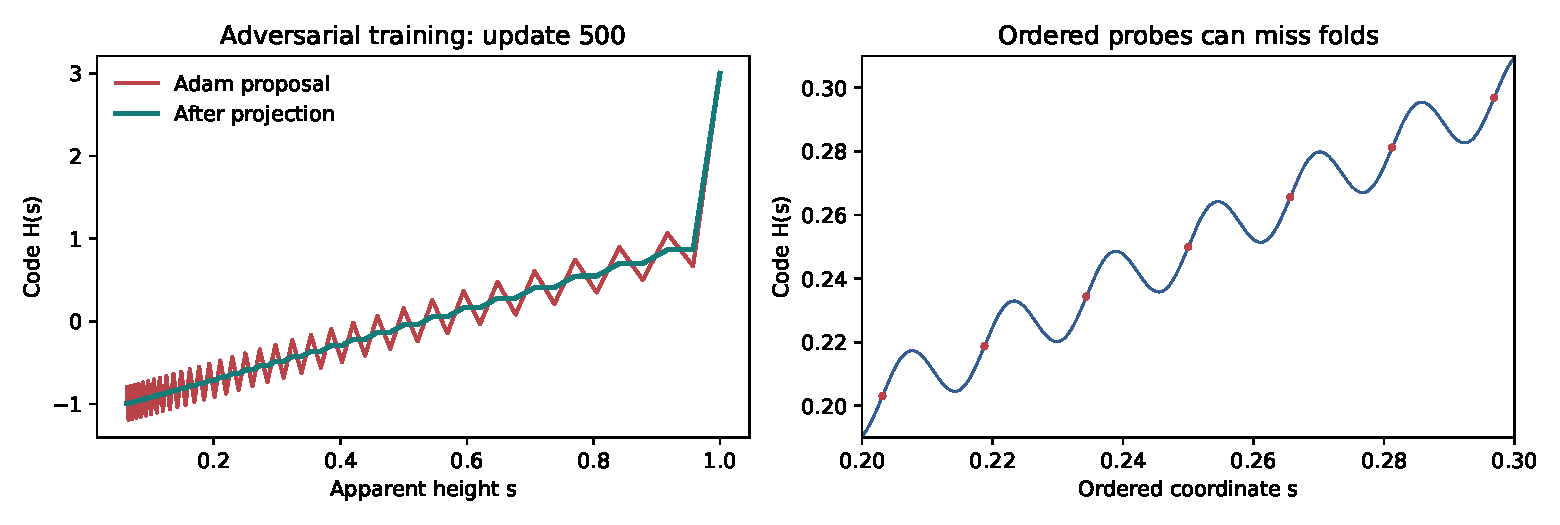
\includegraphics[width=\linewidth]{output/training-stress.pdf}
\end{center}
The right panel evaluates the explicit counterexample \eqref{eq:wiggle}:
red probe values are ordered, but the blue curve reverses between probes.
We also checked PAVA's primal feasibility, dual feasibility, stationarity,
and complementary slackness on 1,000 random input vectors.

\textbf{Finite precision.} The proof is in real arithmetic. The implementation
uses float64, rejects nonfinite losses, requires strictly positive knot
increments, and checks slopes against $.05-10^{-10}$. Rounding can move a
computed slope infinitesimally below $.05$; these checks still leave a
strictly positive margin. They are numerical certificates with tolerances,
not a formal verification of floating-point execution or arbitrary overflow.

\textbf{If the original unrestricted MLP must be kept.} A sufficient
training-only accept/reject rule is possible in principle. For a smooth
curve $h(q)$, assume a \emph{certified} whole-domain bound $|h''(q)|\le L$.
Take a grid including endpoints with maximum gap $\delta$, and one fixed
orientation $\sigma\in\{-1,1\}$. Accept an update only if
\begin{equation}
 \sigma h'(q_i)\ge m+L\delta/2\qquad\text{at every grid point}.
\end{equation}
For any $q$, some grid point is within $\delta/2$. The mean-value bound gives
$\sigma h'(q)\ge\sigma h'(q_i)-L|q-q_i|\ge m>0$.
Starting from a certified feasible model, accepting only certified proposals
and otherwise retaining the old model therefore preserves no-fold.
This may reject every useful step; obtaining a tight bound can be expensive.
This MLP certificate was \emph{not implemented or experimentally tested here}.

\textbf{Reproduction.} From the workspace root, run
\begin{verbatim}
OPENBLAS_NUM_THREADS=1 python3 icm-folding/no-fold-proof/verify.py
cd icm-folding/no-fold-proof
pdflatex -halt-on-error -output-directory=output/pdf no-fold.tex
pdflatex -halt-on-error -output-directory=output/pdf no-fold.tex
\end{verbatim}
\end{document}
